\documentclass{article}



%\usepackage{hyperref}
\usepackage{tikz}
%\usepackage{xcolor}
%\usepackage{amssymb}
\usepackage{wrapfig}
%\usepackage{enumitem}



%\usepackage{geometry}
% \geometry{
% c3paper,
 %total={12in,14in}
% textwidth=12in,
%  textheight=14in,
% showframe
 %}



\begin{document}

\begin{center}

{\bf Dataflow matrix machine}\\
 based on\\
 streams of  V-values\\
 and\\
 variadic neurons.

\vspace{0.4in}

%\begin{wrapfigure}{l}{0.7\textwidth}
%\hspace{0.1in}

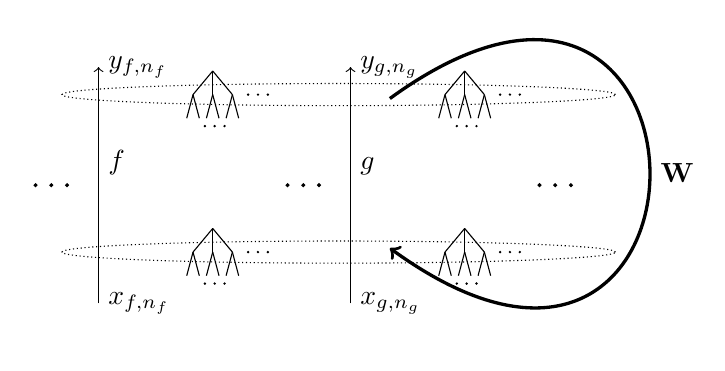
\begin{tikzpicture}
   \clip (-3.5, -2.0) rectangle (5.0, 2.0);

  \filldraw (-3.2,0) circle [radius=0.5pt]
                (-3.0,0)  circle [radius=0.5pt]
                (-3.4, 0) circle [radius=0.5pt]; 

  \draw [->] (-2.6, -1.5) node[right] {$x_{f, n_f}$} -- (-2.6, 1.5) node [midway, above right] {$f$} node[right] {$y_{f, n_f}$};

  \filldraw (0,0) circle [radius=0.5pt]
                (-0.2,0)  circle [radius=0.5pt]
                (0.2, 0) circle [radius=0.5pt];

  \draw [->] (0.6, -1.5) node[right] {$x_{g, n_g}$} -- (0.6, 1.5) node [midway, above right] {$g$} node[right] {$y_{g, n_g}$};

  \filldraw (3.2,0) circle [radius=0.5pt]
                (3.0,0)  circle [radius=0.5pt]
                (3.4, 0) circle [radius=0.5pt]; 


  \draw [->, very thick] (1.1, 1.1) .. controls (5.5, 4.3) and (5.5, -4.0) .. (1.1, -0.8)  node [midway, right] {{\bf W}};

  \foreach \y in {-1.0, 1.0}
    {

      \draw [densely dotted] (0.45, \y+0.15) ellipse [x radius=100pt, y radius=4pt];

     \foreach \x in {-1.0, 2.2}
       {

        \foreach \d in {-0.4, -0.15, 0.1}
           {
               \draw(\x-0.15, \y + 0.45) -- (\x+\d, \y+0.15); 
               \draw (\x+\d, \y + 0.15) -- (\x+\d-0.08, \y-0.15);
               \draw (\x+\d, \y + 0.15) -- (\x+\d+0.08, \y-0.15);
               \filldraw (\x+0.5*\d-0.05, \y-0.25) circle [radius=0.2pt];
               \filldraw (\x+0.5*\d+0.5, \y+0.15) circle [radius=0.2pt];
           }
       } 
     }
 
\end{tikzpicture}

%\caption{``Two-stroke engine" for a DMM based on variadic neurons. Two neurons, $n_f$ and $n_g$, are explicitly pictured.
%Their inputs and outputs, $x_{f, n_f}, x_{g, n_g}, y_{f, n_f},y_{g, n_g}$, are depicted as trees belonging to $U$.
%{\bf W} is a linear map from the concatenation of the first levels of all $y_{h, n_h}$ trees to the concatenation of the first levels of all $x_{h, n_h}$ trees.} 
%\label{fig:dmmnew}
%\end{wrapfigure}

{\tt https://github.com/jsa-aerial/DMM}

\end{center}

%\begin{equation}
$$x_{f, n_f, i}^{t+1} = \sum_{g \in F} \sum_{n_g \in L} \sum_{o \in L} w_{f, n_f, i, g, n_g, o}^t * y_{g, n_g, o}^t$$
%\end{equation}


%\begin{equation}
$$y_{f, n_f}^{t+1} = f(x_{f, n_f}^{t+1})$$
%\end{equation}

%\nopagecolor

%\begin{wrapfigure}{l}{0.7\textwidth}

%\begin{center}


%\vspace*{1.5in}

%\hspace{1in}


%\caption{``Two-stroke engine" for a DMM based on variadic neurons. Two neurons, $n_f$ and $n_g$, are explicitly pictured.
%5Their inputs and outputs, $x_{f, n_f}, x_{g, n_g}, y_{f, n_f},y_{g, n_g}$, are depicted as trees belonging to $U$.
%{\bf W} is a linear map from the concatenation of the first levels of all $y_{h, n_h}$ trees to the concatenation of the first levels of all $x_{h, n_h}$ trees.} 
%\label{fig:dmmnew}
%\end{wrapfigure}

%\end{frame}




\end{document}